\subsection{Materials for the PingaTube}
\label{sec:materials_pingatube}
In order to build the PingaTube detector the following parts were used:
\begin{itemize}
\item a cathod consisting in a aluminium tube (l = 146.5 mm, d$_{inner}$ = 20.63
  mm, d$_{outer}$ = 22.9 mm, d$_{window}$ = 9.2 mm)
\item an anode consisting in a Cu/Be wire (d = 0.025 mm)
\item two bras tubes to prevent gas multiplication at the end of the active
  volume (d = 1 mm, l$_{1}$ = 40.64 mm and l$_{1}$ = 42.72 mm)
\item insulating endcaps
\item P-10 gas Argon (90\%)/CH$_{4}$ (10\%)
\item gas tubes in order to convey the gas (d = 2.1 mm)
\item High voltage (HV) connector in order to supply high voltage to the anode
\item a ground cable in order to connect the cathode
\item O-ring wire connector
\item electric fastenning belt
\item Ultrasound bath with 10/90 Isopropanol/Water
\item Lab tools (Caliper (precition = 1/100 mm), Needle, Gloves, Files, Drill,
  Saw, Microscope, Oscilloscope, etc) and consumables (Soldering flux, aluminium
  tape, epoxy glue, etc)
\end{itemize}

\subsection{Design and Assembly of the PingaTube}
\label{sec:design_and_assembly_beercan}
The main target was to be able to design, build and use in a real data taking
experiment a proportional counter detector using every day objects. Most of the
materials were provided and hence creatively assembling the detector was the
main task. Due to safety regulations some steps, mostly cutting and drilling,
were handled by the instructors.

The bras tubes were sanded at the extremities to avoid sparks that could damage
the anode and, using a microscope, it was verified that no significant notches
were present. Any residue of grease on any of the internal parts could cause
dishomogeneities of the electric field and thus compromise the energy
resolution. In order to prevent this, all the parts were cleaned in an
ultrasonic bath of isopropanol/water mixture.

The thickness of the cathode tube was enough to stop the radiation from the
weaker source of Fe55 thus a small window, that was later covered with a thin
aluminum foil, was opened approximately in the middle of it. Holes were drilled
on plastic endcaps to flush the gas in the active volume and to fit the brass
tubes.

In the assembly phase, the Cu/Be wire was let through the endcaps, the cathode
and the bras tubes which were then put in place in the endcaps. It was then
soldered to a HV connector together with one of the bras tubes on one side and
to the ground on the other. Everything was then sealed using a bi-component
epoxy glue and the cathode was connected to ground.

After the assembly process the P-10 gas was flushed into the detector in order
to extract as much O$_2$ as possible. The main reason for this is that O$_2$ is
a quenching gas that absorbs the avalanche electrons. Leakages of gas from the
detector tube was checked with a flowmeter. The volume of the aluminum tube is
$\approx$ 49~cm$^3$
% \emph{Volume of the tube}, Volume of the tube
% \begin{equation}
%   \label{eq:tube_volume}
%   V=\frac{\pi L^2}{4} =14.65*3.14*2.06324*2.06324=48,96 cm^3
% \end{equation}
With a flow 10 ml/min = 600 cm$^3$/h content of the volume changes ~10 times per
hour. The variation of O$_{2}$ concentration with time is shown on
Figure~\ref{fig:ppm}, it can be seen that the sealing of the detector was
good.
% Units of x-axis are ppm = 1,000,000 m$_{c}$ / m$_{s}$, where m$_{c}$ =
% mass of component (argon/methane mix, kg) m$_{s}$ = mass of solution (oxygen,
% kg).
\begin{figure}[!h]
  \centering
  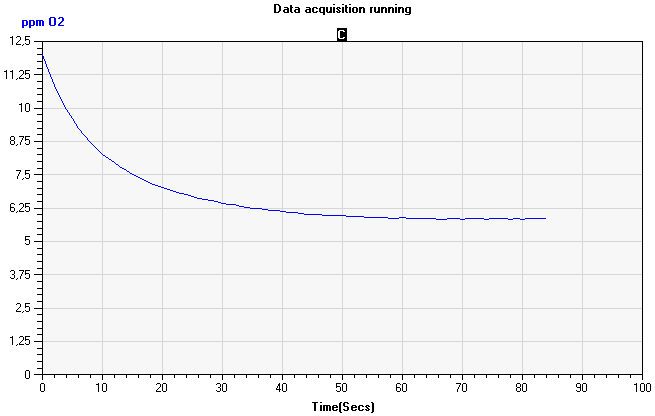
\includegraphics[width=.5\linewidth]{ppm}
  \caption{Variation of O$_2$ concentration as function of time}
  \label{fig:ppm}
\end{figure}

Some problems which were fixed:
\begin{itemize}
\item one of the gas tubes did were not inserted properly which caused gas
  leaking, The problem was sucessfuly fixed afterwards by removing and
  reinserting it properly.  This caused a lot of delay due to the time that the
  glue takes to drying besides the fact that it was needed to reflux the gas on
  the detector.
\item One of the brass tubes slipped inside of the aluminum tube. The issue
  was sorted out on time before the glue dried without any further problem.
\end{itemize}

\subsection{Materials for the BeerCan}
\label{sec:materials_beercan}
In order to build the BeerCan detector the following parts were used:
\begin{itemize}
\item a catode consisting in a beer can (l = 146.5 mm, d$_{inner}$ = 64.0 mm,
  d$_{thickness}$ = 0.2 mm)
\item an anode consisting in a Cu/Be wire (d = 0.075 mm)
\item two bras tubes. (d = 1 mm, l$_{1}$ = 40.64 mm and l$_{1}$ = 42.72 mm)
\item guide in order to protect the brass tubes of touching the can (d = 3.21
  mm)
\item plastic endcaps
\item gas tubes in order to convey the gas (d = 2.1 mm)
\item HV connector in order to supply high voltage to the anode
\item a ground cable in order to connect the cathode.
\item P10 gas Argon (90\%)/CH$_{4}$ (10\%)
\item Ultrasound bath with 10/90 Isopropanol/Water
\item Lab tools (Caliper (precition = 1/100 mm), Needle, Gloves, Files, Drill,
  Saw, Microscope, Oscilloscope, etc) and consumables (Soldering flux, aluminium
  tape, epoxy glue, etc)
\end{itemize}

\subsection{Design and Assembly of the BeerCan}
\label{sec:design_and_assembly_beercan}
The building and assembly was very similar to the description on the PingaTube
detector with the mechanical differences imposed by the beer can geometry.
Again most of the materials were provided and hence creatively assembling the
detector was the main task. After the assembly process the P-10 gas was flushed
into the detector and the flowmeter was used for detecting gas leakages.  Some
differences in the assembly of the BeerCan detector compared to the PingaTube
detector were:
\begin{itemize}
\item Necesity of scratching inner and outer surfaces of the beer can so the
  non-conductive cover was removed.
\item Use of 0.075 mm brass tubes for easier manipulation and insertion of the
  Cu/Be wire.
\end{itemize}
The brass tubes had a diameter of 5.5 mm. The length was chosen so that their
end was at a distance of 3~cm from the center of the can. Further, the diameter
of the gas tubes was 2.86~mm and the length of banana plug was 67~mm.
% Volume of the beercan tube: \emph{Volume of the tube}, Volume of the tube
% \begin{equation}
%   \label{eq:tube_volume}
%   V=\frac{\pi L^2}{4} =14.65*3.14*6.40*6.40=471,05 cm^3
% \end{equation}
With a flow 10 ml/min = 600 cm$^3$/h content of the volume changes ~10 times per
hour.
Some problems that were solved:
\begin{itemize}
\item There was gas leaking in the endcaps, they were sealed by using the epoxy
  glue.
\item The Cu/Be wire got loose while trying to solder it to one of the bras
  tubes which might have caused the detector to have an extremely poor signal
  and was not possible to use it for data taking. There was not enough time for fixing this
  issue due to the lack of time and materials.
\end{itemize}
%%% Local Variables:
%%% mode: latex
%%% TeX-master: "prop_counter"
%%% End:
